% !TeX spellcheck = hu_HU
% !TeX encoding = UTF-8

%----------------------------------------------------------------------------
\chapter{Optimalizációs technikák}\label{chap:optimalization}
%----------------------------------------------------------------------------
Ebben a fejezetben általános optimalizációs technikákat tekintünk át. Történelmi okokból gyakran hívjuk ezeket a technikákat programozásnak, és a felírt formulát programnak, holott természetesen ennek nincs köze ahhoz, amit manapság programozás, illetve program alatt értünk. Ezért is preferálja a modern szakirodalom az optimalizálás szó használatát, de még mindig szinonimaként tekintve a programozást is.

%----------------------------------------------------------------------------
\section{Lineáris optimalizálás}\label{sec:LP}
%----------------------------------------------------------------------------

Egy lineáris optimalizálási (vagy lineáris programozási) probléma  azt jelenti, hogy több keresett mennyiség (úgynevezett változók) lineáris függvényének maximumát vagy minimumát kell meghatározni, mindeközben a rendszerre bizonyos mellékfeltételeket (korlátok) szabunk meg lineáris egyenlőtlenségek vagy egyenletek formájában.
Belátható, hogy a fenti definíciónak megfelelő minden lineáris optimalizálási feladat leírható az alábbi tömör formában, ahol $n$ a változók száma.

Paraméterek:

\begin{tabular}{lll}
	$\mathbf{c}$ & $\in \mathbb{R}^n$   & A célfüggvény együtthatói \\
	$A$ & $\in \mathbb{R}^{m×n}$  & $m × n$-es valós mátrix, a korlátokban szereplő együtthatók \\
	$\mathbf{b}$ & $\in \mathbb{R}^m$   & A korlátokban szereplő konstans tagok \\
\end{tabular}

Változók:

\begin{tabular}{lll}
	$\mathbf{x}$ & $\in \mathbb{R}^n$ & változók \\
\end{tabular}

Célfüggvény:

\begin{align}
	\min_{x} \mathbf{c}^T \mathbf{x} 
\end{align}

Korlátok:

\begin{align}
	A\mathbf{x} \leq \mathbf{b}
\end{align}

A feladat relatív hatékonyan megoldható, ugyan létezik rá polinom idejű algoritmus is, de a gyakorlatban gyakran inkább a Simplex-módszernek elnevezett eljárás valamilyen változatát használják.
A helyzet azonban egészen más, ha a változók nem vehetnek fel bármilyen valós értéket, hanem csak egészek lehetnek. Ekkor a probléma már bizonyítottan NP-nehéz.


%----------------------------------------------------------------------------
\section{Kvadratikus optimalizálás}\label{sec:QuadOpt}
%----------------------------------------------------------------------------

A kvadratikus optimalizálás, vagy kvadratikus programozás a lineáris programozásnál egy általánosabb technika, hiszen megengedi négyzetes tagok jelenlétét a célfüggvényben, amíg a korlátok továbbra is lineárisak.\footnote{Egyes források úgy definiálhatják az általános feladatot, hogy a korlátokban is megengedik négyzetes tagok jelenlétét. Ez szempontunkból most kevésbé lényeges, hiszen a dolgozat jórészt a korlátmentes esetre fókuszál.} Ezzel az alkalmazások körét jóval kibővíti, ugyanakkor az általános feladat megoldása sokkal nehezebbé válik. 

Az általános $n$ változós, $m$ korláttal rendelkező feladatot a következő mátrixos alakban írhatjuk le tömören.

Paraméterek:

\begin{tabular}{lll}
	$Q$ & $\in \mathbb{R}^{n×n}$  & $n × n$-es valós, (szimmetrikus) mátrix, a négyzetes tagok együtthatói \\
	$\mathbf{c}$ & $\in \mathbb{R}^n$   & A lineáris tagok együtthatói \\
	$A$ & $\in \mathbb{R}^{m×n}$  & $m × n$-es valós mátrix, a korlátokban szereplő együtthatók \\
	$\mathbf{b}$ & $\in \mathbb{R}^m$   & A korlátokban szereplő konstans tagok \\
\end{tabular}

Változók:

\begin{tabular}{lll}
	$\mathbf{x}$ & $\in \mathbb{R}^n$ & változók \\
\end{tabular}

Célfüggvény:

\begin{align}
	\min_{\mathbf{x}} \frac{1}{2} \mathbf{x}^T Q \mathbf{x} + \mathbf{c}^T \mathbf{x} 
\end{align}

Korlátok:

\begin{align}
	A\mathbf{x} \leq \mathbf{b}
\end{align}

A felírásnál $Q$ jellemzően egy szimmetrikus mátrix, ekkor a $q_{i,j}$ jelentése, a $x_i \cdot x_j$ változószorzat együtthatója, azonban mivel a pár kétszer is meg fog jelenni, így normálni kell $\frac{1}{2}$-vel. Másik szokásos felírás, hogy $Q$ egy felső háromszög mátrix. Ekkor ha $i \leq j$, akkor $q_{i,j}$ a megfelelő együtthatóval egyezik meg, különben nullával.

A kvadratikus optimalizálást is még lehetséges tovább általánosítani, ha a célfüggvény tetszőlegesen nagy fokszámú polinom is lehet. A kérdés, hogy lehetséges-e ezt az általánosabb problémát visszavezetni a kvadratikus optimalizálás esetére. A válasz nem egyértelmű, de hamarosan egy speciális esetben belátjuk, hogy ez lehetséges.

Több, a kvadratikus optimalizálással rokon optimalizálás fajta is aktívan kutatott tématerület. Ezeknek egyik fő irányvonala a szemidefinit programozás \cite{Ramana1996}. Ugyanakkor a problémának több speciális esete is érdekes lehet. Például tudjuk, hogy ha a $Q$ mátrix szimmetrikus pozitív definit, akkor a probléma ekvivalens a legkisebb négyzetek megkeresésének problémájával, és az optimumot egy lineáris egyenletrendszer megoldásából kaphatjuk \cite{rozsa}.

\section{QUBO}\label{sec:QUBO}

A következőkben a kvadratikus optimalizálás egy speciális esetét fogom elemezni, mely a dolgozat szempontjából is kiemelt jelentőségű, hiszen a munka jelentős része erre fókuszál. Ebben a speciális esetben megkötöm, hogy a változók csak és kizárólag binárisak lehetnek, és több korlát nem adható meg. Mivel a szakirodalom egyszerűen csak QUBO (Quadratic Unconstrained Binary Optimization) néven hivatkozik erre a fajta felírásra \cite{enwiki:1020700695, DWaveOceanBQM}, én is így teszek a továbbiakban.

Bár a probléma rendkívül speciális, gondolhatnánk, hogy akár könnyen megoldható, hiszen csak egy (kvadratikus) polinom maximum- vagy minimumhelyét keressük. Ugyanakkor, mint a későbbi fejezetekben látni fogjuk, több közismerten NP-nehéz feladat visszavezető erre a problémára, így ő maga is NP-nehéz. 

A számunkra érdekes, általános $n$ változós feladat a következő alakban írható fel.

Paraméterek:

\begin{tabular}{lll}
	$Q$ & $\in \mathbb{R}^{n×n}$  & $n × n$-es valós, (szimmetrikus) mátrix, a négyzetes tagok együtthatói \\
	$\mathbf{c}$ & $\in \mathbb{R}^n$   & A lineáris tagok együtthatói \\
\end{tabular}

Változók:

\begin{tabular}{lll}
	$\mathbf{x}$ & $\in \mathbb{B}^n$ & változók \\
\end{tabular}

Célfüggvény:

\begin{align}
	\min_{\mathbf{x}} \frac{1}{2} \mathbf{x}^T Q \mathbf{x} + \mathbf{c}^T \mathbf{x} 
\end{align}

Korlátok:

\begin{align}
	\emptyset
\end{align}

A bináris változók alatt szokásosan 0 vagy 1 értékeket jelölünk, így a továbbiakban is $\mathbb{B}=\{0,1\}$. Ugyanakkor itt érdemes kitérni, hogy bizonyos alkalmazásoknál inkább a $\{-1,1\}$ alaphalmazt tekintik. Erre elterjedt módon Ising-modellként hivatkozhatunk, a fizikai spin irányultságok miatt. Bizonyos esetekben ezt könnyebb lehet elméleti síkon is kezelni, azonban a kettő között (QUBO és Ising-modell) egyszerű lineáris transzformáció ad átjárást, így lényegi különbséget végül nem ad. A D-Wawe Systems gyűjtőnéven BQM-ként (Binary Quadratic Model) hivatkozik a két problémára együttesen \cite{DWaveOceanBQM}.

A továbbiakban feltesszük, hogy a bináris változóink 0 vagy 1 értéket vesznek fel. Ekkor a korábban felírt általános alakot rögtön egyszerűbb alakra hozhatjuk, hiszen bármely változó megegyezik saját négyzetével. Így elég a kvadratikus tagokat felírni, mert az esetleges lineáris tagokat belevehetjük a kvadratikus tagok közé. Továbbá az $\frac{1}{2}$-del való szorzás sem tesz hozzá így már érdemben a felíráshoz, hiszen csak az optimum értékét skálázza, de az optimumhelyek nem változnak. Ennek ellenére az általános felírásban ezen a helyen még benne hagytam.

Paraméterek:

\begin{tabular}{lll}
	$Q$ & $\in \mathbb{R}^{n×n}$  & $n × n$-es valós, (szimmetrikus) mátrix, a négyzetes tagok együtthatói \\
\end{tabular}

Változók:

\begin{tabular}{lll}
	$\mathbf{x}$ & $\in \mathbb{B}^n$ & változók \\
\end{tabular}

Célfüggvény:

\begin{align}
	\min_{x} \frac{1}{2} \mathbf{x}^T Q \mathbf{x}
\end{align}

Korlátok:

\begin{align}
	\emptyset
\end{align}

Fontos megfigyelés lehet még, hogy ha a kvadratikus polinom helyett tetszőlegesen nagy fokszámú polinom szerepelhet a célfüggvényben, melyet a QUBO sémájára PUBO-nak (Polinomial Unconstrained Binary Optimization) hívhatunk, a probléma mindig átírható klasszikus kvadratikus alakra, amely folyamatot a továbbiakban hívjuk \textit{kvadratizálás}nak. Ezt adja meg formálisan az alábbi definíció, illetve tétel.

\begin{definition}[Kvadratizálhatóság]\label{def:kvadratizalhato}
	Azt mondjuk, hogy egy polinom \textit{kvadratizálható}, ha létezik egy olyan kvadratikus polinom, melynek optimumhelyei megegyeznek az eredeti polinom optimumhelyeivel.
\end{definition}

\begin{allitas}\label{theorem:kvadratizalhato}
	Tetszőleges bináris változós polinom kvadratizálható.
	
	A bizonyítás részleteivel most nem foglalkozunk, de az alapötlet, hogy egyszerűen új változókat kell bevezetni, úgy hogy a fokszámok csökkenjenek, és az új bevezetett változó pedig az általa helyettesített két eredeti változó szorzatával legyen egyenlő. Ez utóbbi kikényszeríthető például \az+\refstruc{sec:theoryLogicalGates+ban} taglalt AND kapu implementálásával.
\end{allitas}
	 
Ezzel persze mind a változók száma, mind a kifejezések hossza rendkívüli módon megnőhet. Ha csak egyszerű mohó módszerrel próbálkozunk, akkor akár exponenciálisan is. Nem ismert, hogy van-e jó stratégia a polinomok fokszámának ilyen módon történő csökkentésére, sőt ez a probléma egy jelenleg is futó kutatás alapkérdése.

Figyeljük meg azt is, hogy az állítás csak a bináris változós polinomokra vonatkozik, az általános (nem bináris változós) polinomok esetéről nem állít semmit.


\section{Korlátolt, illetve korlátmentes programozás} \label{sec:constrainedVSunconstrained}

\Az+\refstruc{sec:QUBO+ban} már használtuk a korlátmentesség fogalmát, \az+\refstruc{sec:QUBOform+ban} pedig röviden látni fogjuk, hogy a kvantumszámítógépek segítségével elméletileg hatékonyan megoldhatóak a QUBO feladatok.

Azonban felmerül a kérdés, hogy miként tudjuk mégis használni a gyakorlatban ezt a technikát, nem szorítja-e meg a kezünket túlságosan az, hogy nem adhatunk meg korlátot, és egy ,,egyszerű" függvény szélsőértékét keressük? A válasz szerencsére nemleges, mely látszik a következő, röviden bemutatott technikából \cite{DBLP:journals/corr/abs-1811-11538}. 

Általánosan elmondható, hogy egy optimalizációs esetben kétféle követelményt állítunk a rendszerrel szemben. Ezek közül az egyik típus az erős (hard) követelmény. Ezek olyan követelmények, melyek teljesülését mindenképpen előírjuk a rendszer számára, mert bármelyiknek a sérülése érvénytelenné tenné az eredményt. Általában ezeket a típusú követelményeket korlátként adjuk hozzá a programozási feladathoz.

A követelmények másik fajtája a gyenge (soft) típus. Ezeket is szeretnénk minél jobban teljesíteni, de nem követeljük meg az összestől egyidejűleg. Ez olykor nem is lenne lehetséges, hiszen elég valószínű egy olyan való életbeli probléma, hogy minden gyenge követelmény hozzávétele inkonzisztenssé tenné a rendszert. (Hiszen nem lehet minden tökéletes.) Ezeket a követelményeket általában igyekszünk az optimalizálandó célfüggvénybe belefogalmazni.

A két követelménytípus megfogalmazása között azonban szerencsére van átjárás. Csak annyiról van szó, hogy az erős követelményeket is bele kell tenni a célfüggvénybe, ehhez egyszerűen csak szorozzuk meg őket valamilyen jó nagy együtthatóval (úgynevezett büntetőtaggal), hogy bármelyik erős követelmény sérülése esetén a minimumtól nagyon távol essen a függvény értéke.
Ezt a technikát én is felhasználom a megoldásokban, a képletekben és kódmintákban $P$ szimbólummal jelölve ezt az alkalmasan megválasztott nagy konstans számot.

Ugyanakkor a büntető konstans(ok) megválasztása koránt sem triviális feladat. Bár elméletileg az eredmény ugyanaz, mégis ha túl nagyra választjuk a büntetőtagot, akkor a nem optimális megoldások nagyon messze esnek az optimálistól, ha túl kicsire, akkor pedig túl közel. Egy heurisztikus elven működő optimalizáló szoftvert mind a két szélsőséges eset hátrányosan befolyásolhat. Hiszen ha a helytelen megoldások túl messze vannak az optimumtól, akkor lehet, hogy rossz helyen keresgetünk, és nem találjuk meg a ,,szűk" kis optimumot, amíg ha túl közel esnek, akkor egy nagyon rossz megoldásra is rámondhatjuk, hogy már ,,elég jó".

Ráadásul az explicit korlátokat a megoldó programok sokkal jobban tudják kezelni, mintha a célfüggvénybe fogalmaznánk bele mindent, mert ez utóbbi meglehetősen ,,ködösít" a megoldó szoftver számára, hiszen nem tud lényegi különbséget tenni a különböző funkciójú változók között. Ez persze nem törvényszerű, mert a konkrét megoldó algoritmuson múlik, azonban általánosságban mégis ez várható, és ezt alátámasztja \az+\refstruc{chap:practice+ban} leírt tapasztalat.

\section{QUBO-k hatékonysága}\label{sec:QUBOform}

Mielőtt belevágnánk konkrét feladatok elemzésébe, érdemes áttekinteni az elméleti és gyakorlati hátterét, hogy miként érdemes QUBO feladatokat megkonstruálni, milyen egyszerű mérőszámokkal írható le egy program, mellyel megbecsülhető, hogy milyen könnyen kezelhető az optimalizálás során, és hogy egyáltalán mi ad gyakorlati jelentőséget ennek a megközelítésnek.

Az egyik legegyszerűbb metrika, mellyel a QUBO-t jellemezhetjük, az a változók száma. Ettől szinte közvetlenül függ maga a program mérete is, hiszen nagyságrendileg legfeljebb a váltózószám négyzetével arányos. Így a változók száma egy nagyon triviális, ugyanakkor egy rendkívül fontos mérőszám lesz, bármilyen megoldó programot is használjunk végül az optimalizálási folyamat elvégzésére.

A változók számán felül fontos, hogy megpróbáljuk jellemezni a változók közötti összefonódások bonyolultságát. A legegyszerűbb, ha ehhez definiáljuk a változók gráfját.

\begin{definition}[Változók gráfja]\label{def:valtozokgrafja}
	Minden QUBO felírás egyértelműen reprezentálható egy irányítatlan, élsúlyozott gráffal, melyben a csúcsok a célfüggvény változóinak felelnek meg, és két csúcs között pontosan akkor van él, ha a változók szorzata megjelenik a célfüggvényben. Az él súlya pedig a változók szorzatának az együtthatója. Ezt hívjuk a változók gráfjának vagy a QUBO gráfjának.
\end{definition}

Fontos megjegyezni, hogy az előbbi definíció nem csak megengedi, hanem el is várja hurokélek létezését, amennyiben egy változó önmagával vett szorzata megjelenik. Ezt persze hurokélek helyett reprezentálhatjuk a csúcsok súlyozásával.

A változók gráfját különböző, a gráfelméletben megszokott alapvető metrikával jellemezhetjük, amely közvetlenül utal a QUBO felírás összetettségére is. Ilyen metrika, a már említett csúcsok száma (vagyis a változók száma), élek száma (hány kvadratikus tag szerepel), maximális fokszám (a legtöbb másik változóval kapcsolatban álló változó hány kvadratikus tagban szerepel), vagy az átlagos fokszám (átlagosan hány kvadratikus tagban szerepel egy változó). Ez utolsó természetesen az élek és csúcsok számából már kiszámolható. A fenti metrikákon felül érdemes lehet még nézni a klikkszámot, minimális lefogó csúcshalmaz méretét, vagy bármely más, a gráf nagyságát vagy bonyolultságát leíró értéket.

Megfigyelhető, hogy amennyiben nem QUBO, hanem PUBO alakban formalizáljuk a feladatot, vagyis kvadratikus tagok helyett megengedjük tetszőlegesen nagy fokszámú tagok jelenlétét, akkor is definiálhatjuk a változók gráfját a fentihez hasonló módon, ám ekkor egy hipergráf keletkezik.

\begin{definition}[Változók hipergráfja]\label{def:valtozokhipergrafja}
	Minden PUBO felírás egyértelműen reprezentálható egy irányítatlan, élsúlyozott gráffal, melyben a csúcsok a célfüggvény változóinak felelnek meg, és egy csúcshalmaz pontosan akkor jelenik meg hiperélként, ha a hozzájuk tartozó változók szorzata megjelenik a célfüggvényben. A hiperél súlya pedig a változók szorzatának az együtthatója. Ezt hívjuk a változók hipergráfjának vagy a QUBO hipergráfjának.
\end{definition}

\Az+\refstruc{theorem:kvadratizalhato} mely szerint minden polinom kvadratizálható új változók bevezetésével, most egy gráfelméleti problémát ad, amely arra keresi a választ, hogy miként érdemes új csúcsokat bevezetni, hogy az eredeti hipergráfot a szokásos értelemben vett gráffá konvertáljuk, miközben nem veszítünk el bizonyos strukturális információkat.


A dolgozatnak nem célja bemutatni részletesen, hogy például a D-Wave gépek miként oldják meg a QUBO feladatokat, hiszen sokkal inkább a QUBO-k megfelelő formalizálásán van a hangsúly. Úgy gondolom, hogy mégis elengedhetetlen ennek rövid áttekintése, hiszen csak így van értelme arról beszélni, hogy milyen, és miért ezen metrikákra szeretnénk optimalizálni egy QUBO feladat formalizálása közben.

A D-Wave által nyújtott megoldás alapvető, elméleti hátterét tekintem csak át, hiszen a dolgozat motivációját is lényegében ez adja. A D-Wave Systems egy 1999-ben alapított kanadai cég, mely elsőként hozott kereskedelmi forgalomba kvantumjelenségeket használó számítógépeket. A kvantumgépeik úgynevezett lehűtéses elv alapján működnek, azaz konkrét számolás vagy heurisztika helyett fizikai folyamatok, pontosabban az energiaminimumra törekvés jelenségétől várjuk a megoldást \cite{Szabo}. 

A számítási modell alapját egy speciális gráfba rendezett fizikai qubitek adják, melyek  egymással a gráf struktúrája szerint vannak kapcsolatban. Ez jellemzően az úgynevezett kiméra vagy az újabb gépeken az úgynevezett pegazus topológia \cite{Chimera, Pegasus}. A gráf éleit és csúcsait egyaránt súlyokkal láthatjuk el. Ha visszagondolunk \az+\refstruc{def:valtozokgrafja+ra}, ez pont egy QUBO feladatnak felel meg. Ezután fizikai folyamatok hatására a rendszer beáll várhatóan a legalacsonyabb energiaszintű állapotra, azaz, amikor a qubitek aszerint vesznek fel 0 vagy 1 értéket, hogy az általuk súlyokkal meghatározott kvadratikus függvény értéke vagyis a hozzájuk tartozó QUBO minimális.

Természetes gondolatnak tűnik tehát a QUBO gráfját reprezentálni a hardveren, azonban ez sajnos általában nem működik direkt módon.
Érdemes megkülönböztetni a fizikai qubiteket, melyeken a tényleges optimalizálás történik, illetve a logikai qubiteket, melyek a QUBO-ban felírt változóknak felelnek meg. A kettő között bijektív leképezés lenne a legjobb, azonban sajnos ez általában nem kivitelezhető, hiszen amíg a logikai qubitek között tetszőleges gráfot definiálhatok (melynek \az+\refstruc{def:valtozokgrafja} adott nevet), addig a fizikai qubitek struktúrája a hardver adottságaiból kifolyólag nagyon kötött. Tehát a logikai qubiteket ügyesen rá kell képezni a fizikai qubitekre, amely folyamatot hívjuk beágyazásnak.
Például a kiméra gráfban a maximális fokszám 6, és lévén páros gráf, már egy háromszöget ($K_3$-at) sem lehet beágyazni új változó bevezetése nélkül. Ekkor a módszer jellemzően az, hogy a fizikai qubitek gráfjában láncokat alakítunk ki, amely fizikai qubiteket köt össze, és ugyanannak a logikai qubitnek, azaz változónak felelnek meg. Szintén az erősen korlátos fokszámból látható, hogy olyan csúcsok beágyazása, melynek nagy a fokszáma gondokat okoz. A módszer itt is láncok létrehozása, azonban ezek még több fizikai qubitet emésztenek fel. Egy teljes gráf beágyazása a fenti okok miatt pedig kimondottan körülményes, így megoldó hardver szempontjából mindenképpen az volna az előnyös, ha a gráf klikkszáma kicsi lenne.

\begin{figure}[!ht]
	\centering
	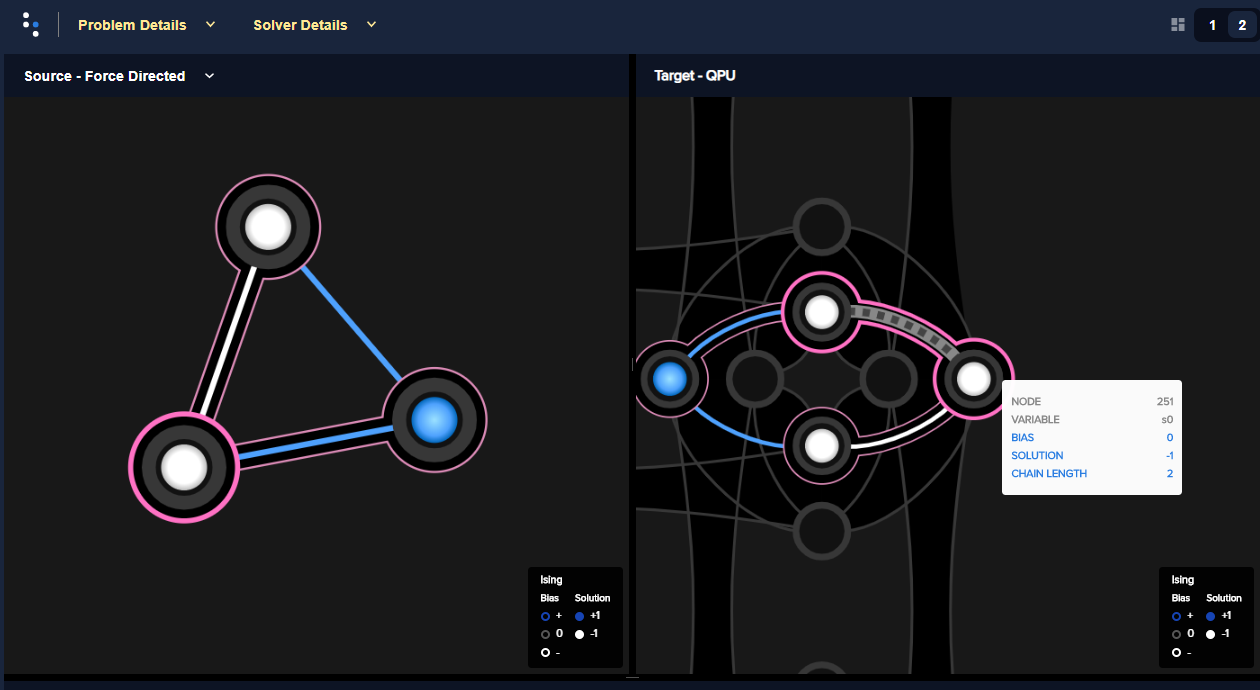
\includegraphics[width=150mm, keepaspectratio]{figures/embedding_3var4qubits.png}
	\caption{$K_3$ beágyazása}
	\label{fig:K3embedding}
\end{figure}

Mint ahogy a \az+\refstruc{fig:K3embedding} is mutatja, a $K_3$ beágyazása úgy lehetséges, ha igénybe veszünk legalább még egy 4. fizikai qubitet, és valamelyik logikai qubit reprezentálásához kettő fizikai qubitet használunk fel, melyek értékét egyenlővé tesszük.

Bár a QUBO problémák beágyazását fizikai hardverre ennél mélyebben a dolgozatban nem vizsgáljuk, fontos észrevétel, hogy igencsak van jelentősége a konstruált QUBO formula és az ahhoz tartozó gráf elemzésének, a korábbi szempontok alapján.